\chapter{脊椎动物胚胎发育}\label{ch:b2:vertebrate-development}

蛙卵是直径两毫米的球体，上方深色，下方浅色。
一天之内，它已分裂成数千个细胞；
两天之内，这些细胞组成的一层沿凹沟卷入内部，
形成原肠，并在背侧铺出一条脊索；三天之内，
脊索上方的细胞层折叠成管，
将发育为脑和脊髓。除水之外，未添加任何物质。
使一个细胞变为游动蝌蚪的信息，
早已存在于卵及其基因组之中；其展开方式——\omterm{def:b2:vertebrate-development:egg}{卵裂}、\omterm{prop:b2:vertebrate-development:gastrulation}{原肠作用}、\omterm{prop:b2:vertebrate-development:neurulation}{神经胚形成}，
以及每个部分受邻近细胞诱导的过程——在鱼、鸡和小鼠中
几乎完全相同。
本章沿着这些步骤考察脊椎动物胚胎的发育，
并介绍那些揭示胚胎各部分如何被告知将成为什么的实验。

\section{从卵到囊胚}

\begin{definition}[卵及其轴]\label{def:b2:vertebrate-development:egg}
\index{动物极}\index{植物极}\index{卵黄}\index{卵裂}
脊椎动物的卵在受精前即已具有极性：
\emph{动物极}含有细胞核和大部分细胞质，
\emph{植物极}则含有\emph{卵黄}，即蛋白质和脂质的贮存物，
胚胎将依靠它生活，直至能够取食。卵黄的多少
决定了此后一切发育的模式：海胆或哺乳动物的卵几乎没有卵黄，
发生完全卵裂，形成大小相等的细胞；蛙卵卵黄量适中，
同样发生完全卵裂，但为不等分裂（上方为小细胞，下方为富含卵黄的大细胞）；
鱼卵或鸟卵几乎全是卵黄，
卵裂仅发生在其上方的一片胞质盘中。
在蛙卵中，精子进入的位置决定了第二条轴：
皮层从该点转开三十度，暴露出
与进入点相对的\emph{灰色新月}，该侧将
发育为背侧。\emph{卵裂}是一系列快速有丝分裂，
无生长，每次分裂后细胞体积减半，由卵中储存的母源
mRNA 和蛋白质驱动，胚胎自身的基因
保持沉默，直至\emph{\omterm{def:b2:vertebrate-development:blastula}{囊胚}中期转换}，
即约十二次分裂之后。
\end{definition}

\begin{omfigure}
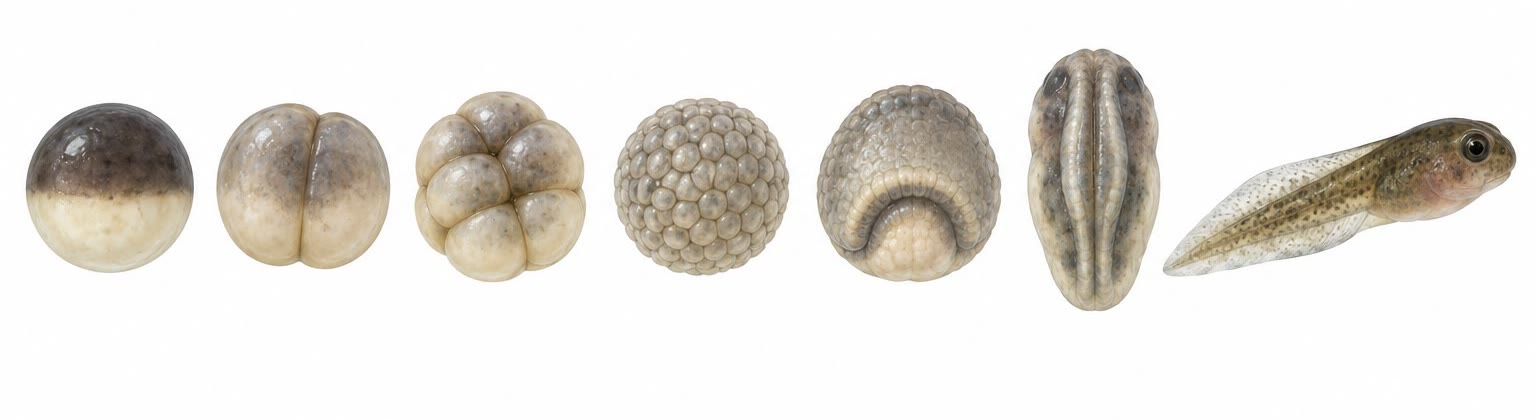
\includegraphics[width=0.9\linewidth]{images/book4/ai/b4-10-frog-development.jpg}

{\small 蛙受精卵的发育过程：由\omterm{def:b2:vertebrate-development:egg}{卵裂}形成\omterm{def:b2:vertebrate-development:blastula}{囊胚}，
经\omterm{prop:b2:vertebrate-development:gastrulation}{原肠作用}形成带神经褶的神经胚，以及
蝌蚪——全部过程仅需数天，且无生长。}
\end{omfigure}

\begin{theorem}[卵裂的算术]\label{thm:b2:vertebrate-development:cleavage}
经过 $k$ 次同步\omterm{def:b2:vertebrate-development:egg}{卵裂}后，体积为 $V_0$ 的卵变为 $2^{k}$
个细胞，每个细胞的平均体积为 $V_0/2^{k}$，半径为 $r_0/2^{k/3}$，并且
总表面积增大为原来的 $2^{k/3}$ 倍；核体积与细胞质体积之比
在蛙卵中起始约为 $10^{-4}$，
此后增为原来的 $2^{k}$ 倍，约十次分裂后达到普通细胞的数值（$\sim 0.1$）。
正是这一上升的比值——一定量母源抑制剂
被指数增长的 DNA 量所滴定——触发了\omterm{def:b2:vertebrate-development:blastula}{囊胚}中期转换：
分裂减慢、不再同步，
合子基因组
随之开启。
\end{theorem}
\begin{proof}
\omterm{def:b2:vertebrate-development:egg}{卵裂}过程中体积守恒，因此 $2^{k}$ 个细胞中每个的体积为 $V_0
2^{-k}$，视为球体，半径为 $r_0 2^{-k/3}$；其总面积为
$2^{k}\cdot 4\pi r_0^{2}\, 2^{-2k/3} = 4\pi r_0^{2}\, 2^{k/3}$。每个
细胞保留一个大小固定的细胞核，因此比值按 $2^{k}$ 倍增加，
由 $10^{-4}$ 出发，$2^{10} = 1024$ 使其达到 $0.1$。蛙的\omterm{def:b2:vertebrate-development:blastula}{囊胚}中期
转换发生在第十二次分裂，
与稍后达到的阈值相一致。
\end{proof}
\begin{proof}[证据]
纽波特和柯什纳（1982）向蛙卵中加入额外的 DNA，并
发现转换提前出现，提前的分裂次数与
DNA 过量的程度相当；去除细胞质也产生同样效果。这个“时钟”
并非时间，也不是分裂次数，而是一个比值。
\end{proof}

\begin{definition}[囊胚]\label{def:b2:vertebrate-development:blastula}
\index{囊胚}\index{囊胚腔}
\omterm{def:b2:vertebrate-development:egg}{卵裂}结束时形成\emph{囊胚}：一个中空的球体（蛙、海胆）
或由数千个细胞构成的圆盘（鱼、鸟），围绕一个腔，即
\emph{囊胚腔}。其细胞外观上尚未特化，
但彼此并不等同：通过对表面的若干小块染色并追踪，
所作的\emph{命运图}表明：
动物帽将发育为皮肤和神经系统（\emph{外胚层}），
赤道带发育为肌肉、骨骼、肾和血液
（\emph{中胚层}），\omterm{def:b2:vertebrate-development:egg}{植物极}一侧的细胞团则发育为肠及其器官
（\emph{内胚层}）。这三个\emph{胚层}在各种脊椎动物中都相同，
下一步是把它们安置到各自的位置：
中胚层和内胚层位于外侧，必须内移。
\end{definition}

\section{原肠作用与神经胚形成}

\begin{proposition}[原肠作用]\label{prop:b2:vertebrate-development:gastrulation}
\index{原肠作用}\index{胚孔}\index{原肠}\index{脊索}
\emph{\omterm{prop:b2:vertebrate-development:gastrulation}{原肠作用}}是使单层的\omterm{def:b2:vertebrate-development:blastula}{囊胚}
转变为三层的\emph{原肠胚}的一组细胞运动。在蛙中，
它始于灰色新月下方：该处细胞改变形状，
其外端收缩成瓶状，表面内陷形成凹沟，
即\emph{\omterm{prop:b2:vertebrate-development:gastrulation}{胚孔}}。中胚层和内胚层经此向内
流入（\emph{内卷}），越过唇缘，
沿\omterm{def:b2:vertebrate-development:blastula}{囊胚腔}顶部向前移动；动物帽
向下延展覆盖外表（\emph{外包}）；\omterm{prop:b2:vertebrate-development:gastrulation}{胚孔}
闭合成环，围绕最后的富含\omterm{def:b2:vertebrate-development:egg}{卵黄}的细胞。内部形成
一个以内胚层为衬里的新腔，即\emph{原肠}，是未来的肠道，
而最先内卷的中胚层沿中线
形成一根硬杆，即\emph{脊索}，是每个脊椎动物胚胎的轴，
也是该门得名的结构。在鸟类和哺乳动物中，
同样的运动在扁平的胚盘上通过一条狭缝（\emph{原条}）进行，
在鱼中，胚盘在\omterm{def:b2:vertebrate-development:egg}{卵黄}上延展。
这些运动的编排随\omterm{def:b2:vertebrate-development:egg}{卵黄}而异；结果——外胚层位于外侧，
内胚层衬于肠道，中胚层居中，脊索位于中线
——是相同的。
\end{proposition}

\begin{omfigure}
\begin{tikzpicture}[every node/.style={font=\scriptsize}, >=stealth]
  % blastula
  \begin{scope}
    \draw[thick, fill=omDef!15] (0,0) circle (1.3);
    \draw[thick, fill=white] (0,0.2) circle (0.75);
    \fill[omExo!40] (0,0) ++(-1.3,0) arc (180:360:1.3 and 1.3) -- cycle;
    \draw[thick] (0,0) circle (1.3);
    \node at (0,0.2) {囊胚腔};
    \node[below, align=center] at (0,-1.45) {囊胚 \\动物极帽（蓝色），富含卵黄的细胞（灰色）};
  \end{scope}
  % early gastrula: blastopore forming
  \begin{scope}[xshift=4.2cm]
    \draw[thick, fill=omDef!15] (0,0) circle (1.3);
    \draw[thick, fill=white] (0,0.25) circle (0.7);
    \fill[omExo!40] (0,0) ++(-1.3,0) arc (180:360:1.3 and 1.3) -- cycle;
    \draw[thick] (0,0) circle (1.3);
    \draw[very thick, omThm] (1.0,-0.85) .. controls (0.5,-0.6) and (0.4,-0.3) .. (0.55,0.0);
    \draw[->, thick, omThm] (1.15,-0.7) .. controls (0.6,-0.4) .. (0.4,0.1);
    \draw[omThm] (1.0,-0.85) -- (0.9,-1.25); \node[omThm, anchor=north west] at (0.6,-1.2) {胚孔唇};
    \node[below, align=center] at (0,-1.45) {早期原肠胚 \\细胞越过唇缘内卷};
  \end{scope}
  % late gastrula
  \begin{scope}[xshift=8.4cm]
    \draw[thick, fill=omDef!15] (0,0) circle (1.3);
    \draw[thick, fill=omExo!25] (0,0.05) circle (0.95);
    \draw[thick, fill=white] (0.15,-0.1) ellipse (0.55 and 0.4);
    \draw (0.6,-0.3) -- (1.6,-1.15); \node[anchor=west] at (1.6,-1.15) {原肠};
    \draw[very thick, omThm] (-0.9,0.35) .. controls (-0.2,0.6) .. (0.8,0.4);
    \draw[omThm] (0.0,0.48) -- (-0.9,1.55); \node[omThm, anchor=east] at (-0.9,1.55) {脊索};
    \draw[thick] (1.1,-0.7) -- (1.3,-0.5);
    \node[right] at (1.3,-0.5) {胚孔};
    \node[below, align=center] at (0,-1.45) {晚期原肠胚：三个胚层、\\肠腔，以及位于肠顶的脊索};
  \end{scope}
\end{tikzpicture}

{\small 青蛙原肠胚切面。细胞越过\omterm{prop:b2:vertebrate-development:gastrulation}{胚孔}唇
向内卷入；内胚层衬于新的肠腔，而
最先进入的中胚层沿中线形成脊索。}
\end{omfigure}

\begin{proposition}[神经胚形成与身体构型]\label{prop:b2:vertebrate-development:neurulation}
\index{神经胚形成}\index{神经管}\index{体节}\index{神经嵴}
脊索上方的外胚层增厚为\emph{神经
板}，其边缘隆起成褶，在中线处汇合，形成
\emph{\omterm{prop:b2:vertebrate-development:neurulation}{神经管}}，即未来的脑和脊髓，它
沉入皮肤之下；褶皱顶部的细胞，即
\emph{\omterm{prop:b2:vertebrate-development:neurulation}{神经嵴}}，迁移离开，形成外周神经、
色素细胞、肾上腺髓质及大部分面部。
脊索两侧，中胚层分节为块，即
\emph{\omterm{prop:b2:vertebrate-development:neurulation}{体节}}，自头至尾逐对出现，它们形成
椎骨、躯干肌和真皮；侧中胚层
分化为衬于体腔的各层，并形成心脏和
四肢；内胚层管芽生出肺、肝和胰。
\omterm{prop:b2:vertebrate-development:neurulation}{神经胚形成}结束时，胚胎已具备脊椎动物的身体构型
——背侧神经索位于脊索之上，腹侧为消化道，分节的
肌肉，有头部——此时长约数毫米，其后的
发育即是在此构型上细化各器官
（见\cref{ch:b2:limb-organogenesis}）。
\end{proposition}

\begin{omfigure}
\begin{tikzpicture}[every node/.style={font=\scriptsize}]
  \foreach \x/\lab in {0/{神经板}, 4.0/{神经褶隆起}, 8.0/{神经管闭合；神经嵴细胞迁移}} {
    \begin{scope}[xshift=\x cm]
      \draw[thick, fill=omExo!25] (-1.6,0) rectangle (1.6,-1.6);
      \draw[thick, omThm, fill=omThm!30] (0,-0.75) circle (0.28);
      \draw[thick, fill=omProp!30] (-1.3,-0.75) circle (0.32); \draw[thick, fill=omProp!30] (1.3,-0.75) circle (0.32);
      \node[below, align=center, text width=3.4cm] at (0,-1.7) {\lab};
    \end{scope}
  }
  \draw[very thick, omDef] (-1.6,0) -- (-0.7,0) .. controls (-0.3,0.15) and (0.3,0.15) .. (0.7,0) -- (1.6,0);
  \draw[very thick, omDef] (2.4,0) -- (3.3,0) .. controls (3.3,0.9) and (3.6,0.1) .. (4.0,0.0) .. controls (4.4,0.1) and (4.7,0.9) .. (4.7,0) -- (5.6,0);
  \draw[very thick, omDef] (6.4,0.05) -- (9.6,0.05);
  \draw[very thick, omDef, fill=omDef!20] (8.0,-0.3) circle (0.3);
  \foreach \p in {(7.35,-0.4),(8.65,-0.4)} \fill[omDef!70!black] \p circle (0.07);
  \node[omThm, anchor=west] at (9.8,-0.75) {脊索};
  \node[omProp, anchor=west] at (9.8,-1.15) {体节};
  \node[omDef, anchor=west] at (9.8,-0.3) {神经管};
  \node[omDef!70!black, anchor=west] at (9.8,0.1) {神经嵴细胞};
\end{tikzpicture}

{\small \omterm{prop:b2:vertebrate-development:neurulation}{神经胚形成}的横切面：脊索上方的外胚层
脊索（红色）增厚、褶叠并闭合为\omterm{prop:b2:vertebrate-development:neurulation}{神经管}
（蓝色），脊索旁的中胚层分节为
\omterm{prop:b2:vertebrate-development:neurulation}{体节}（橙色），\omterm{prop:b2:vertebrate-development:neurulation}{神经嵴}细胞离开闭合中的褶。}
\end{omfigure}

\begin{omfigure}
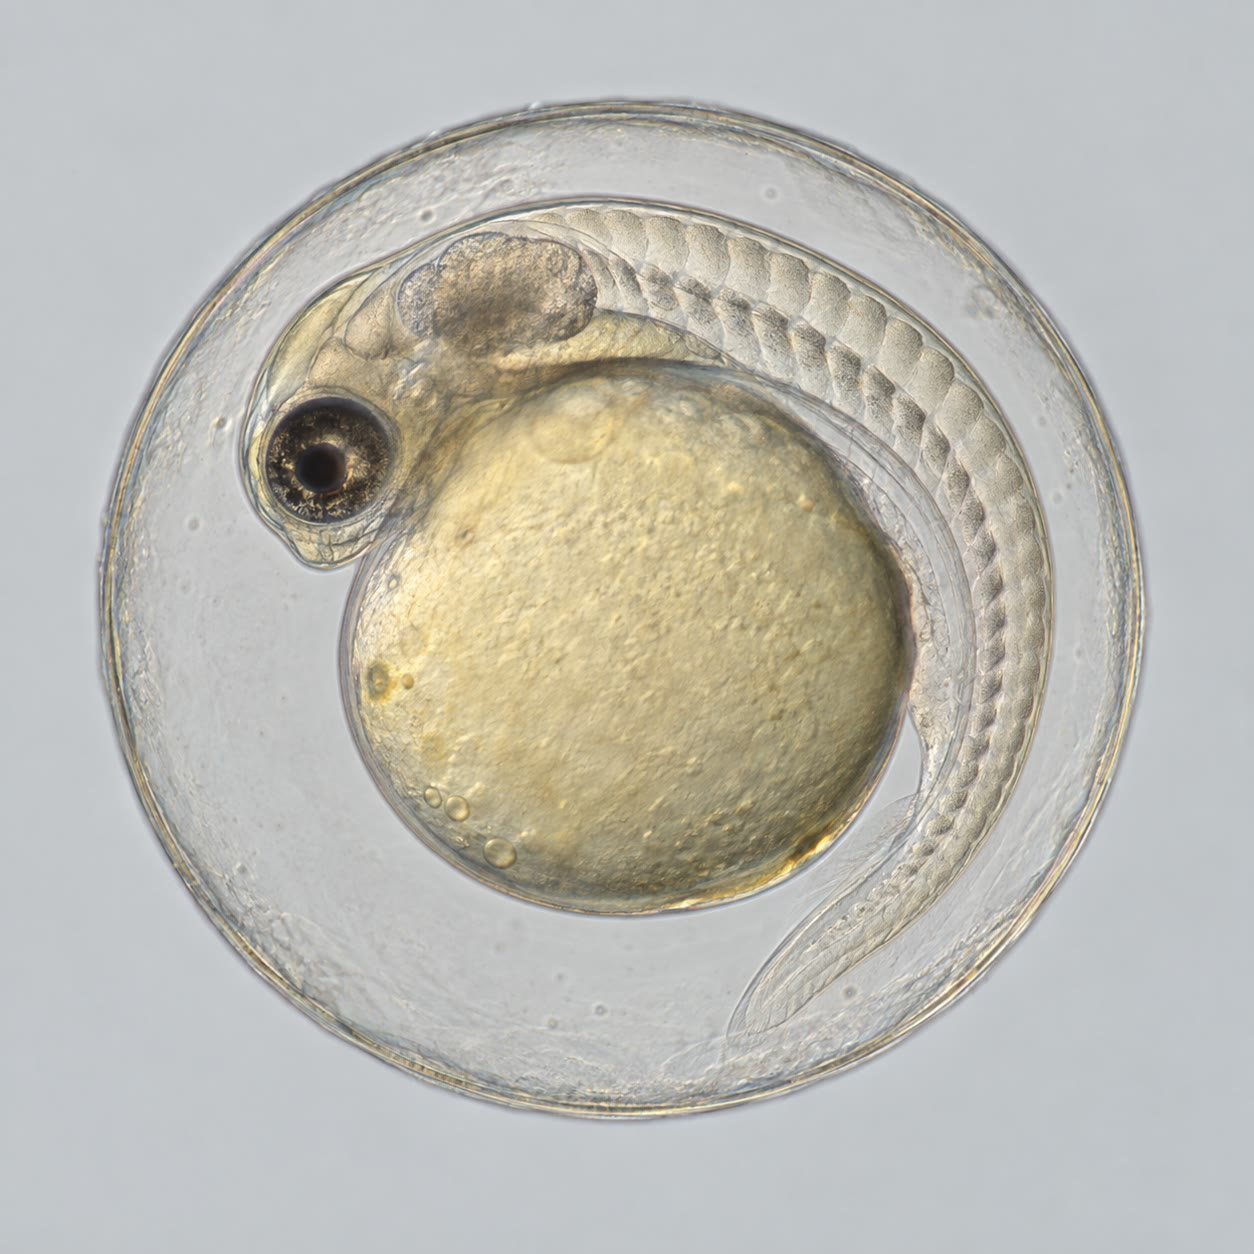
\includegraphics[width=0.42\linewidth]{images/book4/ai/b4-10-zebrafish-embryo.jpg}\hspace{0.04\linewidth}
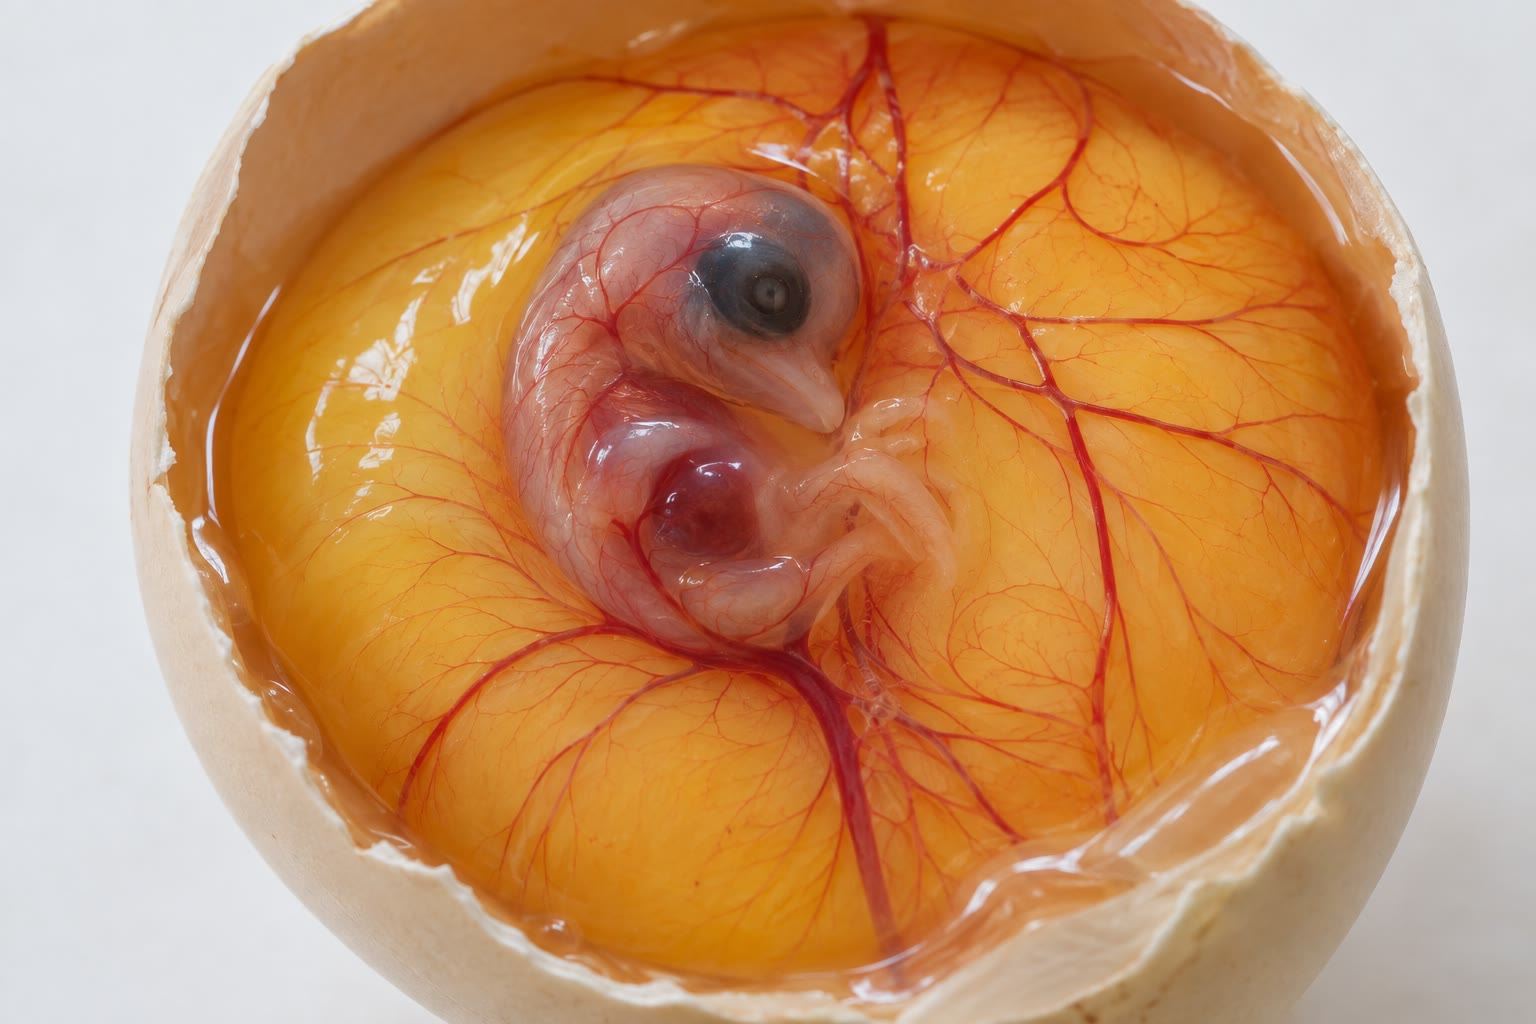
\includegraphics[width=0.5\linewidth]{images/book4/ai/b4-10-chick-embryo.jpg}

{\small 左：一日龄斑马鱼胚胎，位于卵膜内，
蜷绕在\omterm{def:b2:vertebrate-development:egg}{卵黄}周围，可见眼、脑和一排\omterm{prop:b2:vertebrate-development:neurulation}{体节}。
右：三日龄鸡胚，位于\omterm{def:b2:vertebrate-development:egg}{卵黄}上，心脏已
开始搏动，血管在\omterm{def:b2:vertebrate-development:egg}{卵黄}上铺展，以汲取其中营养。}
\end{omfigure}

\section{诱导：细胞如何知道自己的位置}

\begin{definition}[诱导与感受态]\label{def:b2:vertebrate-development:induction}
\index{诱导（胚胎）}\index{感受态}\index{组织者}
\emph{诱导}是一组细胞借助信号改变
邻近另一组细胞命运的过程；应答的细胞
必须具有\emph{感受态}——即能够应答，而这种能力
只在有限的时间内存在。发育是一连串的诱导：\omterm{def:b2:vertebrate-development:egg}{植物极}
细胞诱导其上方的细胞形成中胚层；背侧中胚层
——即\omterm{prop:b2:vertebrate-development:gastrulation}{胚孔}唇处的\emph{组织者}——诱导其上方的
外胚层形成神经板，并使两侧中胚层
形成相应模式；脊索诱导\omterm{prop:b2:vertebrate-development:neurulation}{神经管}底板；
视泡是脑的芽体，诱导其所接触的皮肤
形成晶状体；晶状体诱导角膜。每一被诱导的组织又成为
下一步的诱导者。信号是若干反复使用的分泌性蛋白质家族
——同样的信号塑造
肢体（见\cref{ch:b2:limb-organogenesis}），并在成体中驱动
信号传导（在\cref{ch:b2:cell-signalling}中）。
\end{definition}
\begin{proof}[证据]
施佩曼与曼戈尔德（1924）切下一种蝾螈早期原肠胚的背侧\omterm{prop:b2:vertebrate-development:gastrulation}{胚孔}唇，
并将其移植到另一种蝾螈的腹侧，
两者色素不同，以便能区分宿主细胞与移植细胞。
移植体并未简单地变成它在原位本会成为的样子：
它向内卷入，形成脊索，并
\emph{诱导宿主自身的腹侧外胚层}形成第二条
\omterm{prop:b2:vertebrate-development:neurulation}{神经管}，并在其旁形成宿主的\omterm{prop:b2:vertebrate-development:neurulation}{体节}——一个完整的第二胚胎，
主要由宿主细胞组成，与第一个胚胎腹对腹相连。
原肠胚的其他任何部分都无法做到这一点。他们将该唇
称为\omterm{def:b2:vertebrate-development:induction}{组织者}；其信号（阻断腹侧化因子 BMP 的蛋白质）
于七十年后被鉴定。
\end{proof}

\begin{omfigure}
\begin{tikzpicture}[every node/.style={font=\scriptsize}, >=stealth]
  % donor
  \draw[thick, fill=omDef!12] (0,0) circle (1.3); \node[above] at (0,1.4) {供体原肠胚（浅色）};
  \draw[very thick, omThm] (0.85,-0.95) arc (-45:-20:1.3); \node[omThm, right] at (1.2,-0.8) {背唇};
  \draw[->, thick] (1.6,-0.3) -- (3.4,-0.3);
  % host
  \draw[thick, fill=omExo!45] (5,0) circle (1.3); \node[above] at (5,1.4) {宿主原肠胚（深色）};
  \draw[very thick, omThm] (5.85,-0.95) arc (-45:-20:1.3); \node[omThm, right] at (6.2,-0.8) {自身的唇};
  \draw[very thick, omThm] (4.15,0.95) arc (135:160:1.3); \node[omThm, left] at (3.9,1.0) {移植体};
  \draw[->, thick] (6.6,-0.3) -- (8.4,-0.3);
  % result: twinned embryo
  \draw[thick, fill=omExo!45] (10.6,0) ellipse (1.8 and 1.1);
  \draw[very thick, omDef!70!black] (9.2,0.5) .. controls (10.0,0.8) and (11.2,0.8) .. (12.0,0.5);
  \draw[very thick, omDef!70!black] (9.2,-0.5) .. controls (10.0,-0.8) and (11.2,-0.8) .. (12.0,-0.5);
  \node[above] at (10.6,1.2) {结果：两条轴};
  \node[anchor=north, align=center, text width=4cm] at (10.6,-1.2) {由移植体诱导、由\emph{宿主}细胞构成的第二条神经管和体节};
\end{tikzpicture}

{\small \omterm{def:b2:vertebrate-development:induction}{组织者}实验。将背唇移植到另一原肠胚的腹侧，
诱导宿主细胞形成第二条
胚轴。}
\end{omfigure}

\begin{theorem}[形态发生素梯度]\label{thm:b2:vertebrate-development:gradient}
\index{形态发生素}
许多诱导通过\emph{\omterm{thm:b2:vertebrate-development:gradient}{形态发生素}}实现：由源头分泌的一种信号，
在组织中扩散，细胞依据其局部浓度读取该信号——
高于某一阈值时为一种命运，高于更高阈值时为
另一种命运。设\omterm{thm:b2:vertebrate-development:gradient}{形态发生素}在平面源处以速率
每单位面积 $j$ 产生，扩散系数为 $D$，并以速率
$k$ 降解，则稳态时其浓度呈指数分布
\[
c(x) = c_0\,e^{-x/\lambda}, \qquad \lambda = \sqrt{D/k}, \qquad c_0 = \frac{j}{\sqrt{Dk}},
\]
因此，浓度降至阈值 $T$
以下的距离为 $x_T = \lambda\ln(c_0/T)$：组织可借助
固定阈值被划分为宽度固定的条带。取 $D =
\qty{1e-12}{m^2/s}$（一种在组织中移动时因结合而减慢的蛋白质）；
及 $k = \qty{1e-3}{s^{-1}}$（半衰期约为十二
分钟），则 $\lambda = \sqrt{10^{-9}}\,\unit{m} \approx
\qty{32}{\micro m}$：约几个细胞直径，
即胚胎场被图式化所跨越的尺度。加倍源强度会使
$c_0$ 加倍，并使每个边界向外移动 $\lambda
\ln 2$。
\end{theorem}
\begin{proof}
稳态时扩散与降解相平衡：$D\,c'' = k\,c$，
其衰减解为 $c = c_0 e^{-x/\lambda}$，其中 $\lambda^2 =
D/k$。离开源的通量为 $-Dc'(0) = Dc_0/\lambda = j$，
由此得 $c_0 = j\lambda/D = j/\sqrt{Dk}$。令 $c(x_T) = T$
即得 $x_T$；将 $c_0$ 换为 $2c_0$ 则使其增加 $\lambda\ln 2$。
\end{proof}

\begin{omfigure}
\begin{tikzpicture}
\begin{axis}[
  width=0.78\linewidth, height=5.6cm,
  axis x line=bottom, axis y line=left,
  xmin=0, xmax=120, ymin=0, ymax=1.1,
  xlabel={距源的距离（\unit{\micro m}）}, ylabel={形态发生素（相对值）},
  xlabel style={font=\small, at={(axis description cs:0.5,-0.13)}, anchor=north},
  ylabel style={font=\small},
  tick label style={font=\small}, xtick={0,32,64,96}, ytick={0,0.5,1},
  clip=false,
]
\fill[omThm!18] (axis cs:0,0) rectangle (axis cs:22,1.05); \node[font=\scriptsize, anchor=south] at (axis cs:11,1.05) {命运 A};
\fill[omProp!18] (axis cs:22,0) rectangle (axis cs:61,1.05); \node[font=\scriptsize, anchor=south] at (axis cs:41,1.05) {命运 B};
\fill[omExo!18] (axis cs:61,0) rectangle (axis cs:120,1.05); \node[font=\scriptsize, anchor=south] at (axis cs:90,1.05) {命运 C};
\addplot[very thick, omDef, domain=0:120, samples=80] {exp(-x/32)};
\draw[dashed, gray] (axis cs:0,0.5) -- (axis cs:22,0.5) -- (axis cs:22,0);
\draw[dashed, gray] (axis cs:0,0.15) -- (axis cs:61,0.15) -- (axis cs:61,0);
\node[font=\scriptsize, anchor=west] at (axis cs:62,0.55) {阈值 1};
\node[font=\scriptsize, anchor=west] at (axis cs:62,0.2) {阈值 2};
\end{axis}
\end{tikzpicture}

{\small 当 $\lambda = \qty{32}{\micro m}$ 时的\omterm{thm:b2:vertebrate-development:gradient}{形态发生素}梯度。
两个阈值将组织划分为三个细胞命运条带，其
宽度由 $\lambda$ 以及阈值与源浓度之比
决定。}
\end{omfigure}

\begin{example}[读取梯度]\label{ex:b2:vertebrate-development:reading}
在蛙原肠胚中，暴露于不同剂量激活素家族信号的边缘区细胞，
随剂量由高到低分别成为脊索、肌肉、肾和血液；
置于培养皿中、带有阈值剂量开关的解离动物帽细胞，
其命运在浓度相差两倍之内即发生改变。
在\omterm{prop:b2:vertebrate-development:neurulation}{神经管}中，来自脊索和底板的信号
向上扩散，并自底部依次决定运动神经元，
随后是各类中间神经元，
其阈值相隔几个细胞直径。
生物体的坐标以浓度来书写。
\end{example}

\section{命运、决定及决定的时机}

\begin{proposition}[细胞命运何时固定]\label{prop:b2:vertebrate-development:commitment}
\index{决定}\index{胚胎调节}
细胞的\emph{命运}是它通常会成为的类型；其
\emph{潜能}是它被移动后可能成为的类型；
当其命运不再随周围环境改变时，即称其为\emph{已决定的}。
早期胚胎具有\emph{调节}能力：蛙的前两个
\omterm{def:b2:vertebrate-development:egg}{卵裂}球被分离后，各自都能发育为一个完整的小蝌蚪，
哺乳动物胚胎的最初细胞也都是全能的——同卵双胞胎
正是由此产生。决定的过程是逐渐的，
不同组织的决定时间各不相同：将一小块早期原肠胚的
外胚层移植到腹侧，它会成为腹部皮肤；而取自晚期原肠胚的同一片段，
无论放在何处都会形成神经板；
到尾芽期，移植到侧腹的肢区会在该处形成
肢体。相比之下，在大多数无脊椎动物中，命运在早期
即由每个细胞所继承的细胞质固定（\emph{镶嵌}发育），
被分离的\omterm{def:b2:vertebrate-development:egg}{卵裂}球只能形成其自身所属的那一部分。脊椎动物的策略
是保持细胞的可塑性，通过诱导告诉细胞该做什么——
正是这一策略使双胞胎、再生和\omterm{def:b2:vertebrate-development:induction}{组织者}实验
成为可能。
\end{proposition}
\begin{proof}[证据]
施佩曼（1901）在两细胞期用一根毛发圈套住一枚蝾螈卵：
若毛圈位于灰色新月所在的平面内，使每一半都得到其一部分，
则形成两个完整的胚胎；若毛圈与之垂直，
使一半拥有整个新月，则该半形成一个胚胎，
另一半则形成一团腹部组织。
新月——即未来的\omterm{def:b2:vertebrate-development:induction}{组织者}——是唯一不能
被分割的部分。
\end{proof}

\begin{example}[青蛙的发育时间表]\label{ex:b2:vertebrate-development:timetable}
在 \qty{18}{\celsius} 下：受精；第一次\omterm{def:b2:vertebrate-development:egg}{卵裂}在 \qty{1.5}{h}，
此后每半小时一次；\num{4000} 个细胞的\omterm{def:b2:vertebrate-development:blastula}{囊胚}形成于 \qty{7}{h}；
\omterm{def:b2:vertebrate-development:blastula}{囊胚}中期转换在 \qty{8}{h}；原肠胚形成于 \qty{10}{h} 至
\qty{20}{h}；神经褶在 \qty{30}{h} 时闭合；心脏开始搏动于
\qty{2.5}{d}；孵化并开始摄食于 \qty{4}{d}，此时为
体长 \qty{6}{mm} 的蝌蚪。斑马鱼一天内完成同样过程，鸡需三天，
小鼠需九天；人类胚胎在第三周形成原肠胚，并
在第四周内闭合\omterm{prop:b2:vertebrate-development:neurulation}{神经管}——此时多数女性尚不知自己
已经怀孕，这正是为何\omterm{prop:b2:vertebrate-development:neurulation}{神经管}闭合所需的叶酸
须在受孕前即行补充。
\end{example}

\section{练习}

\begin{exercise}[$\star$]\label{exo:b2:vertebrate-development:1}
定义\omterm{def:b2:vertebrate-development:egg}{卵裂}、\omterm{def:b2:vertebrate-development:blastula}{囊胚}、原肠胚形成和\omterm{prop:b2:vertebrate-development:neurulation}{神经胚形成}，并指出
每个阶段产生的结构。
\end{exercise}

\begin{exercise}[$\star$]\label{exo:b2:vertebrate-development:2}
给出三个胚层，并对每一胚层列出由它发育而来的
四种成体组织。
\end{exercise}

\begin{exercise}[$\star$]\label{exo:b2:vertebrate-development:3}
\omterm{def:b2:vertebrate-development:egg}{卵黄}的多少如何改变\omterm{def:b2:vertebrate-development:egg}{卵裂}与原肠胚形成的
模式？试比较青蛙与鸡。
\end{exercise}

\begin{exercise}[$\star$]\label{exo:b2:vertebrate-development:4}
什么是诱导？按在青蛙胚胎中发生的先后顺序给出三次诱导，
并分别指出诱导物与应答组织。
\end{exercise}

\begin{exercise}[$\star\star$]\label{exo:b2:vertebrate-development:5}
半径为 \qty{1}{mm} 的青蛙卵经过十二次\omterm{def:b2:vertebrate-development:egg}{卵裂}。计算
细胞数、细胞的平均半径，以及细胞总表面积增大的
倍数。胚胎为何需要
额外增加的表面积？
\end{exercise}

\begin{exercise}[$\star\star$]\label{exo:b2:vertebrate-development:6}
核质比起始值为 $10^{-4}$，而
\omterm{def:b2:vertebrate-development:blastula}{囊胚}中期转换发生于其达到 $0.4$ 时。经过多少次
分裂？若向卵内注入相当于其自身三倍量的
DNA，转换将出现在第几次分裂时？
\end{exercise}

\begin{exercise}[$\star\star$]\label{exo:b2:vertebrate-development:7}
\omterm{thm:b2:vertebrate-development:gradient}{形态发生素}的扩散系数为 $D = \qty{2e-12}{m^2/s}$，半衰期为
\qty{10}{min}。计算 $k$ 与 $\lambda$。两个阈值分别位于
源浓度的 \qty{50}{\%} 和 \qty{10}{\%} 处，求出
三个命运带的宽度。
\end{exercise}

\begin{exercise}[$\star\star$]\label{exo:b2:vertebrate-development:8}
在上一题的梯度中，源浓度因一次
\omterm{def:b2:genome-diversification:mutation}{突变}而加倍。各边界分别移动多少？若
改为降解速率加倍，又会如何？
\end{exercise}

\begin{exercise}[$\star\star$]\label{exo:b2:vertebrate-development:9}
描述施佩曼–曼戈尔德实验，说明两个物种为何
必须在色素上存在差异，并指出该结果排除了什么。
\end{exercise}

\begin{exercise}[$\star\star\star$]\label{exo:b2:vertebrate-development:10}
预测下列操作的结果：(a) 将早期原肠胚的一小块预定神经板
移植到腹部；(b) 取自晚期原肠胚的同一小块，
同样移植到腹部；(c) 将一小块腹部外胚层覆盖在
晚期原肠胚的脊索上；(d) 从早期
原肠胚中切除整个\omterm{def:b2:vertebrate-development:induction}{组织者}。试用\omterm{def:b2:vertebrate-development:induction}{感受态}和决定
的概念分别解释每一结果。
\end{exercise}

\begin{exercise}[$\star\star\star$]\label{exo:b2:vertebrate-development:11}
青蛙的第一次\omterm{def:b2:vertebrate-development:egg}{卵裂}需 \qty{90}{min}，其后十一次\omterm{def:b2:vertebrate-development:egg}{卵裂}各需
\qty{30}{min}，均在 \qty{18}{\celsius} 下进行；在 \qty{10}{\celsius} 时每一步都
慢 2.5 倍。两种温度下，\omterm{def:b2:vertebrate-development:blastula}{囊胚}中期转换分别
在何时达到？试说明为何转换
在两种温度下都出现在相同的细胞数，这说明了什么
关于发育时钟？
\end{exercise}

\begin{exercise}[$\star\star\star$]\label{exo:b2:vertebrate-development:12}
“脊椎动物胚胎靠对话构建，无脊椎动物胚胎
靠遗传构建。”讨论调节性发育与镶嵌性发育的对比，
它们对孪生与再生的影响，以及
二者为何只是程度上的差异。
\end{exercise}

\section{问题：青蛙胚胎的计时与模式形成}

\begin{problem}[{周末问题——跟踪青蛙胚胎
贯穿卵裂、囊胚中期转换、原肠胚形成与诱导的过程，
计算形态发生素梯度，预测经典移植实验的结果，
结尾于转换时的细胞数与时间，以及
命运带的宽度}]
\label{pb:b2:vertebrate-development:1}
青蛙卵的半径为 \qty{0.7}{mm}，细胞核半径为
\qty{0.03}{mm}，其 DNA 含量为 $c$；每次\omterm{def:b2:vertebrate-development:egg}{卵裂}需
\qty{30}{min}，第一次\omterm{def:b2:vertebrate-development:egg}{卵裂}需 \qty{75}{min}。\omterm{def:b2:vertebrate-development:blastula}{囊胚}中期
转换发生在总 DNA 量达到 $4000\,c$ 时。\omterm{thm:b2:vertebrate-development:gradient}{形态发生素}的扩散系数为 $D =
\qty{1e-12}{m^2/s}$，半衰期为 \qty{20}{min}，源浓度为
$c_0$，阈值位于 $0.4\,c_0$ 与 $0.08\,c_0$ 处。

\medskip
\noindent\textbf{第一部分——\omterm{def:b2:vertebrate-development:egg}{卵裂}。}
\begin{enumerate}
  \item 计算卵及其细胞核的体积，以及
        初始核质比。
  \item DNA 量经几次\omterm{def:b2:vertebrate-development:egg}{卵裂}后达到 $4000\,c$？
        此时共有多少个细胞？
  \item 受精后经过多长时间？
  \item 此时细胞的平均半径是多少，若细胞核保持原有大小，
        则核体积与细胞体积之比为多少？请加以评述。
  \item 细胞总表面积增大了多少倍？
  \item 每次\omterm{def:b2:vertebrate-development:egg}{卵裂}都需复制基因组：共合成了多少 DNA，
        以 $c$ 为单位，并解释为何胚胎
        在此过程中无需转录其基因？
  \item 转换时发生了什么变化，以及哪一实验
        表明它是由比值而非细胞数所触发的？
\end{enumerate}

\medskip
\noindent\textbf{第二部分——原肠胚形成。}
\begin{enumerate}[resume]
  \item \omterm{prop:b2:vertebrate-development:gastrulation}{胚孔}相对于精子进入点形成于何处，
        由什么决定了该位置？
  \item 按顺序列出经\omterm{prop:b2:vertebrate-development:gastrulation}{胚孔}卷入的组织，
        以及它们随后所处的位置。
  \item 原肠胚形成耗时 \qty{10}{h}，内卷的细胞层
        移动了 \qty{2}{mm}。求细胞的平均速度，
        以微米每分钟表示，并与爬行的
        成纤维细胞（\qty{1}{\micro m/min}）比较。
  \item 为什么原肠胚形成不能
        在\omterm{def:b2:vertebrate-development:blastula}{囊胚}中期转换之前发生？
  \item 用一句话说明，为什么脊索而非\omterm{prop:b2:vertebrate-development:neurulation}{神经管}
        是脊索动物的定义性结构。
  \item 在原肠胚形成开始时施用阻断细胞形状改变的药物，
        预测胚胎的结果。
\end{enumerate}

\medskip
\noindent\textbf{第三部分——梯度。}
\begin{enumerate}[resume]
  \item 由半衰期求 $k$，并求 $\lambda$。
  \item 求两个阈值的位置。
  \item 给出三个命运区带的宽度，分别以微米和
        长度为 \qty{15}{\micro m} 的细胞数表示。
  \item 源的强度减半。重新计算两个位置，并说明
        哪一个区带缩小最多。
  \item 距源 \qty{60}{\micro m} 处的细胞，
        分别考虑在读取梯度之前被移至 \qty{10}{\micro m} 处和读取之后被移动的情形；
        两种情形下它各变为什么？为什么？
  \item 说明指数分布的浓度剖面为何使边界位置
        依赖于源强度的对数，
        以及这为何使模式形成具有稳健性。
\end{enumerate}

\medskip
\noindent\textbf{第四部分——移植。}
\begin{enumerate}[resume]
  \item 预测将背唇移植到早期原肠胚的腹侧，
        以及将腹侧边缘区移植到背侧，
        两者的结果各如何。
  \item 预测将背唇移植到
        \emph{神经胚}的腹侧，并解释二者的差异。
  \item 将二细胞期的蛙胚沿灰色新月所在的
        平面切开；另一次则沿与之垂直的平面切开。预测
        两种情形的结果。
  \item 从\omterm{def:b2:vertebrate-development:blastula}{囊胚}上切下动物帽，单独培养；
        同一动物帽也可与\omterm{def:b2:vertebrate-development:egg}{植物极}细胞并置培养。预测
        所形成的组织。
  \item 施佩曼和曼戈尔德的结果为何要求宿主与移植体
        必须可以区分，若移植的是错误的物种，
        则会表明什么？
  \item 给出结果：转换时的\omterm{def:b2:vertebrate-development:egg}{卵裂}次数和时间、
        其细胞数，以及三个区带的宽度。
\end{enumerate}
\end{problem}
